\documentclass[landscape]{article}

\usepackage{tboxen}
\usepackage{amsmath}
\usepackage{amssymb}
\usepackage{epsfig}
\usepackage[tight]{subfigure}
\usepackage{color}
\usepackage{type1cm}
\usepackage{subfig}

% Custom variables

% How much length we want to add to the poster while editing.  Note
% that these are just integer variables.  There is probably a better
% way to do this...
\newcounter{width}
\newcounter{height}
\newcounter{extra-length}
\setcounter{width}{90} % developing at 50% magnification of 6' x 4' poster
\setcounter{height}{60}
\setcounter{extra-length}{0}
%\setcounter{extra-length}{30} % for development

% Boolean variable: whether or not we want to show grid lines
\newif\ifusegrid
%\usegridtrue
\usegridfalse

% You can define any rgb colors you want for the background.  The
% first two lines define a blue to cream fade.  See how they are used
% below.
\definecolor{topcolor}{rgb}{0.05,0.30,0.57}
\definecolor{bottomcolor}{rgb}{1, 1, 1}
% Uncomment these next two lines if you want to have an all white background.
% TODO: temp dev setting
\definecolor{topcolor}{rgb}{1,1,1}
\definecolor{bottomcolor}{rgb}{1,1,1}

% Other counters that we will use below.
\newcounter{grid-top}
\newcounter{grid-right}
\newcounter{title-top}
\newcounter{title-left-margin}
\newcounter{title-width}
\newcounter{title-left}
\newcounter{title-box-width}

% ==============================================================================
% Set up paper sizes

\newcounter{total-height}
\setcounter{total-height}{\arabic{height} + \arabic{extra-length}}
\setlength{\paperwidth}{\arabic{width}cm}
\setlength{\paperheight}{\arabic{total-height}cm}
\setlength{\textwidth}{\paperwidth}
\setlength{\textheight}{\paperheight}

% These usually stay the same for tboxen
\setlength{\headheight}{0 cm}
\setlength{\headsep}{0 cm}
\setlength{\topmargin}{-2 cm} 
\setlength{\oddsidemargin}{-1in}

% From tboxen:
% this is often necessary for pdf and dvips to work
\ifx\pdfoutput\undefined 
% for dvi
\special{papersize=\arabic{width}cm,\arabic{height}cm}
\else 
% for pdf
\pdfpagewidth=\paperwidth 
\pdfpageheight=\paperheight 
\fi 

% ==============================================================================
% POSTER STARTS HERE
\begin{document}
\begin{center}
  
  % ==============================================================================
  % Main body
  \begin{tikzpicture}
    
    % This defines your background box - entries are pretty self explanatory.
    % The colors ``topcolor'' and ``bottomcolor'' are defined above.
    \shade[top color = topcolor,
      bottom color = bottomcolor,
      rounded corners = 1cm, % The larger this is, the rounder your corners
      line width = 2mm, % The width of your border lines
      draw]
    (0,0) rectangle +(\textwidth-2cm,\textheight-1cm); 
    % This last line above just sets up the bounding box for the whole poster.  You don't want to change it.

    % ==============================================================================
    \ifusegrid
    % Draw grid guidelines if desired.
    \setcounter{grid-top}{\arabic{total-height}-1}
    \setcounter{grid-right}{\arabic{width}-2}
    \draw[style=help lines] (0,\arabic{extra-length}) grid (\arabic{grid-right},\arabic{grid-top});
    \setcounter{grid-top}{\arabic{height}-1}
    \foreach \x in {0,5,...,\arabic{grid-right}}
    \foreach \y in {0,5,...,\arabic{grid-top}}
    \draw (\x,\y) + (0,\arabic{extra-length}) node{\tiny \x,\y};
    \fi

    % ==============================================================================
    % Title box
    %
    % The following defaults make the title box span the whole top,
    % start 3cm from the top, and end 2 cm from both sides. I have
    % hard-coded the 2s and 3 below.  Play around with the trade-off
    % between changing these numbers and changing
    % ``title-left-margin'' if you are not happy with the defaults.
    \setcounter{title-left-margin}{0} % This specifies the additional padding to the right and left of the title.  Can be negative.
    \setcounter{title-top}{\arabic{total-height}-3} % Places the top of the title 3 cm from the top of the poster.
    \setcounter{title-width}{\arabic{width}-2*\arabic{title-left-margin} - 2*2 - 4} % Automatically calculates the width of the title based on the margin.
    \setcounter{title-left}{\arabic{title-left-margin} + 2} % Automatically places the title 2m from the left edge of the poster + the user specified margin.
    \setcounter{title-box-width}{\arabic{width} - 30}
    \path (\arabic{title-left},\arabic{title-top}) node(title) [style=tbox, text width=\arabic{title-width}cm] {
      \begin{center}
        % Three parboxes allow for images on both sides of the title
        % box with the title text in the middle.
        \parbox{5cm} {
        
\includegraphics[width=5cm]{../../figures/berkeley_seal.pdf}
        }
        \parbox{\arabic{title-box-width}cm} {
          \centering
              {\huge \bf{Object Detection on a Budget} } \\
              \vspace{1cm}
              \begin{tabular}{cccc}
                {\Large Sergey Karayev, \hfill} & {\Large Mario Fritz, \hfill} & {\Large Pieter Abbeel, \hfill} & {\Large Trevor Darrell}\\
                \multicolumn{4}{c}{\large Ongoing Work at UC Berkeley and MPI Informatics}
              \end{tabular}
        }
        \parbox{5cm} {
          
\includegraphics[width=5cm]{../../figures/minerva.pdf}
        }
      \end{center}
    };
    
    % ==============================================================================
    % LEFT COLUMN
    \path (title.south west) ++(0cm,-2cm) + (-\arabic{title-left-margin}cm,0cm) node(introduction) [style=tbox,text width=23cm] {
    \begin{itemize}
    \item The most common approach to state-of-the-art object detection is through repeated classification of image windows.
    \item Classifier operates on a global template feature or assemblage of local features.
    \end{itemize}
    \begin{center}
        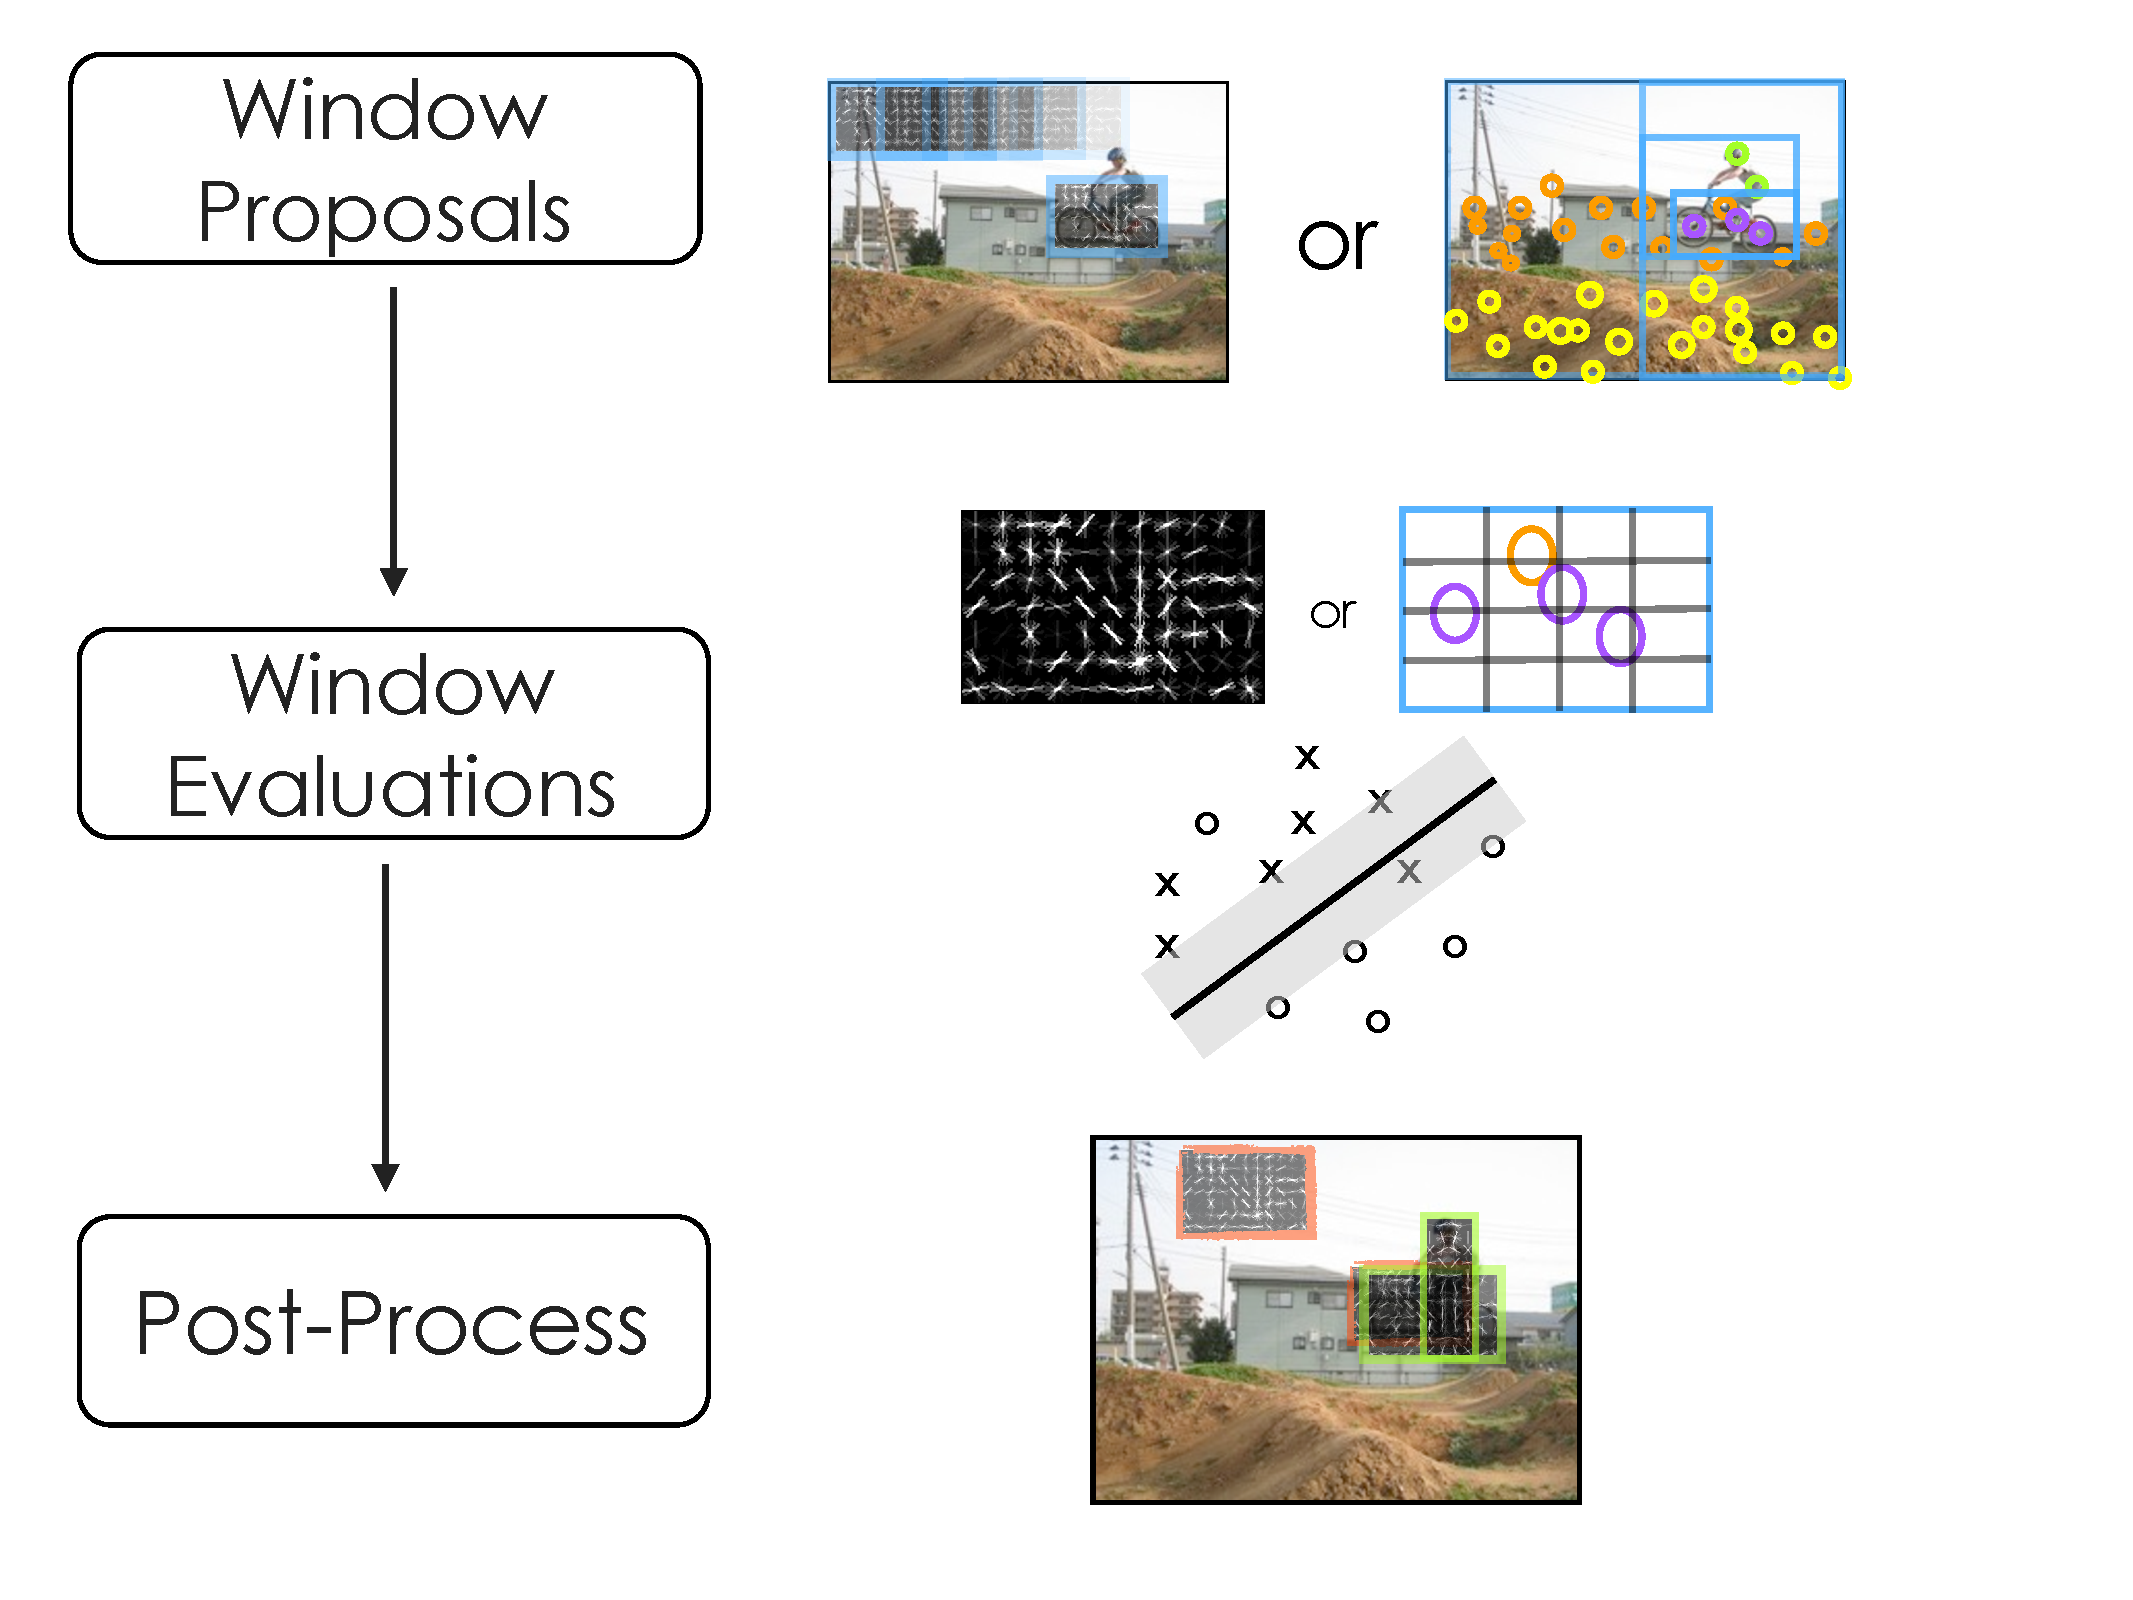
\includegraphics[width=22cm]{../../figures/detection.pdf}
      \end{center}
    }; \addcenteredtitle{introduction}{Object Detection} 
    
    % ==============================================================================
    \path (introduction.south west) ++(0cm,-2cm) node(efficient) [style=tbox,text width=23cm] {
    \begin{itemize}
    \item The \emph{window proposal} stage can be made faster with 
      \begin{itemize}
        \item a pre-filtering step that proposes only a small subset of all possible windows (e.g. ``Objectness'' 2010)
        \item an algorithmically efficient way to pick subwindows to process (e.g. Branch \& Bound 2008, Branch \& Rank 2011)
      \end{itemize}
      
    \item The \emph{window evaluation} stage can be made faster with a cascaded classifier, which rejects low-likelihood windows quickly (e.g. Viola-Jones detector, 2004).

    \item Window proposals are key to really make a difference---fast classifiers with exhaustive windows are not as efficient.
    \end{itemize}
    \begin{center}
      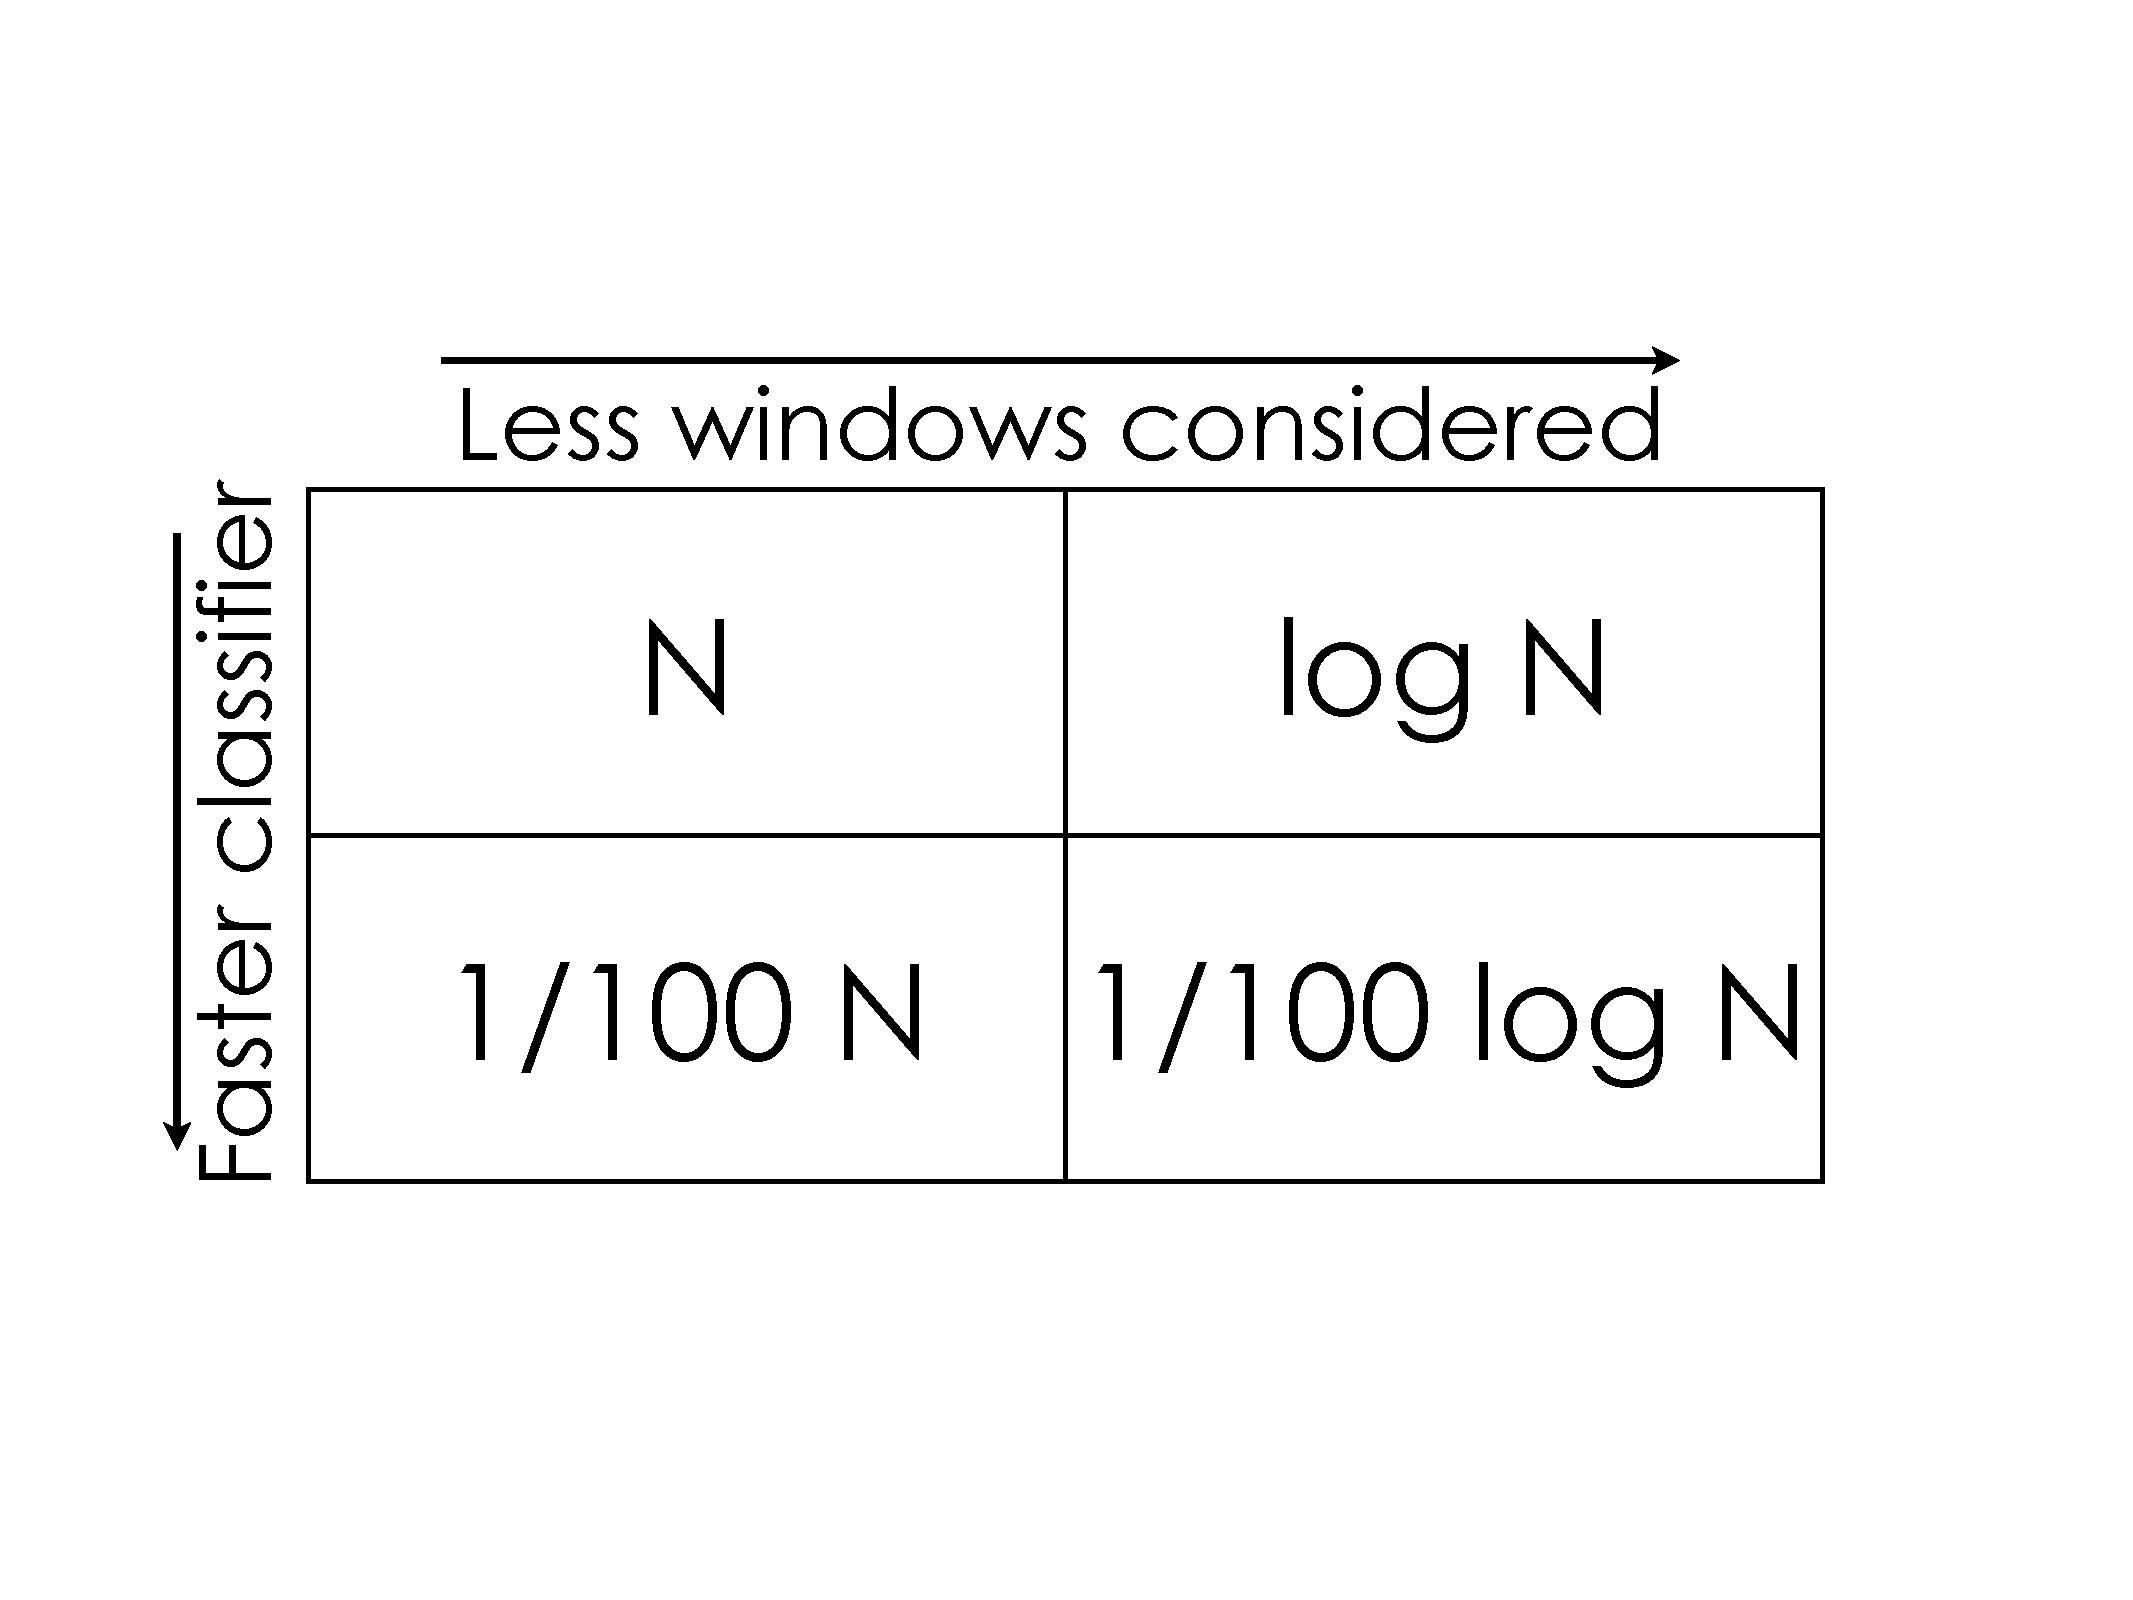
\includegraphics[width=10cm]{../../figures/fast_vs_efficient.pdf}
    \end{center}

    }; \addcenteredtitle{efficient}{Efficiency and Speed}

    % ==============================================================================
    % CENTER COLUMN 
    \path (introduction.north east) ++(2cm,0cm) node(budget) [style=tbox,text width=26cm] {
    \begin{itemize}
      \item If we need to maintain a certain framerate, or have a large dataset to process in a fixed amount of time, we can only allot a small amount of time to each image.
    \end{itemize}
    
      \begin{center}
        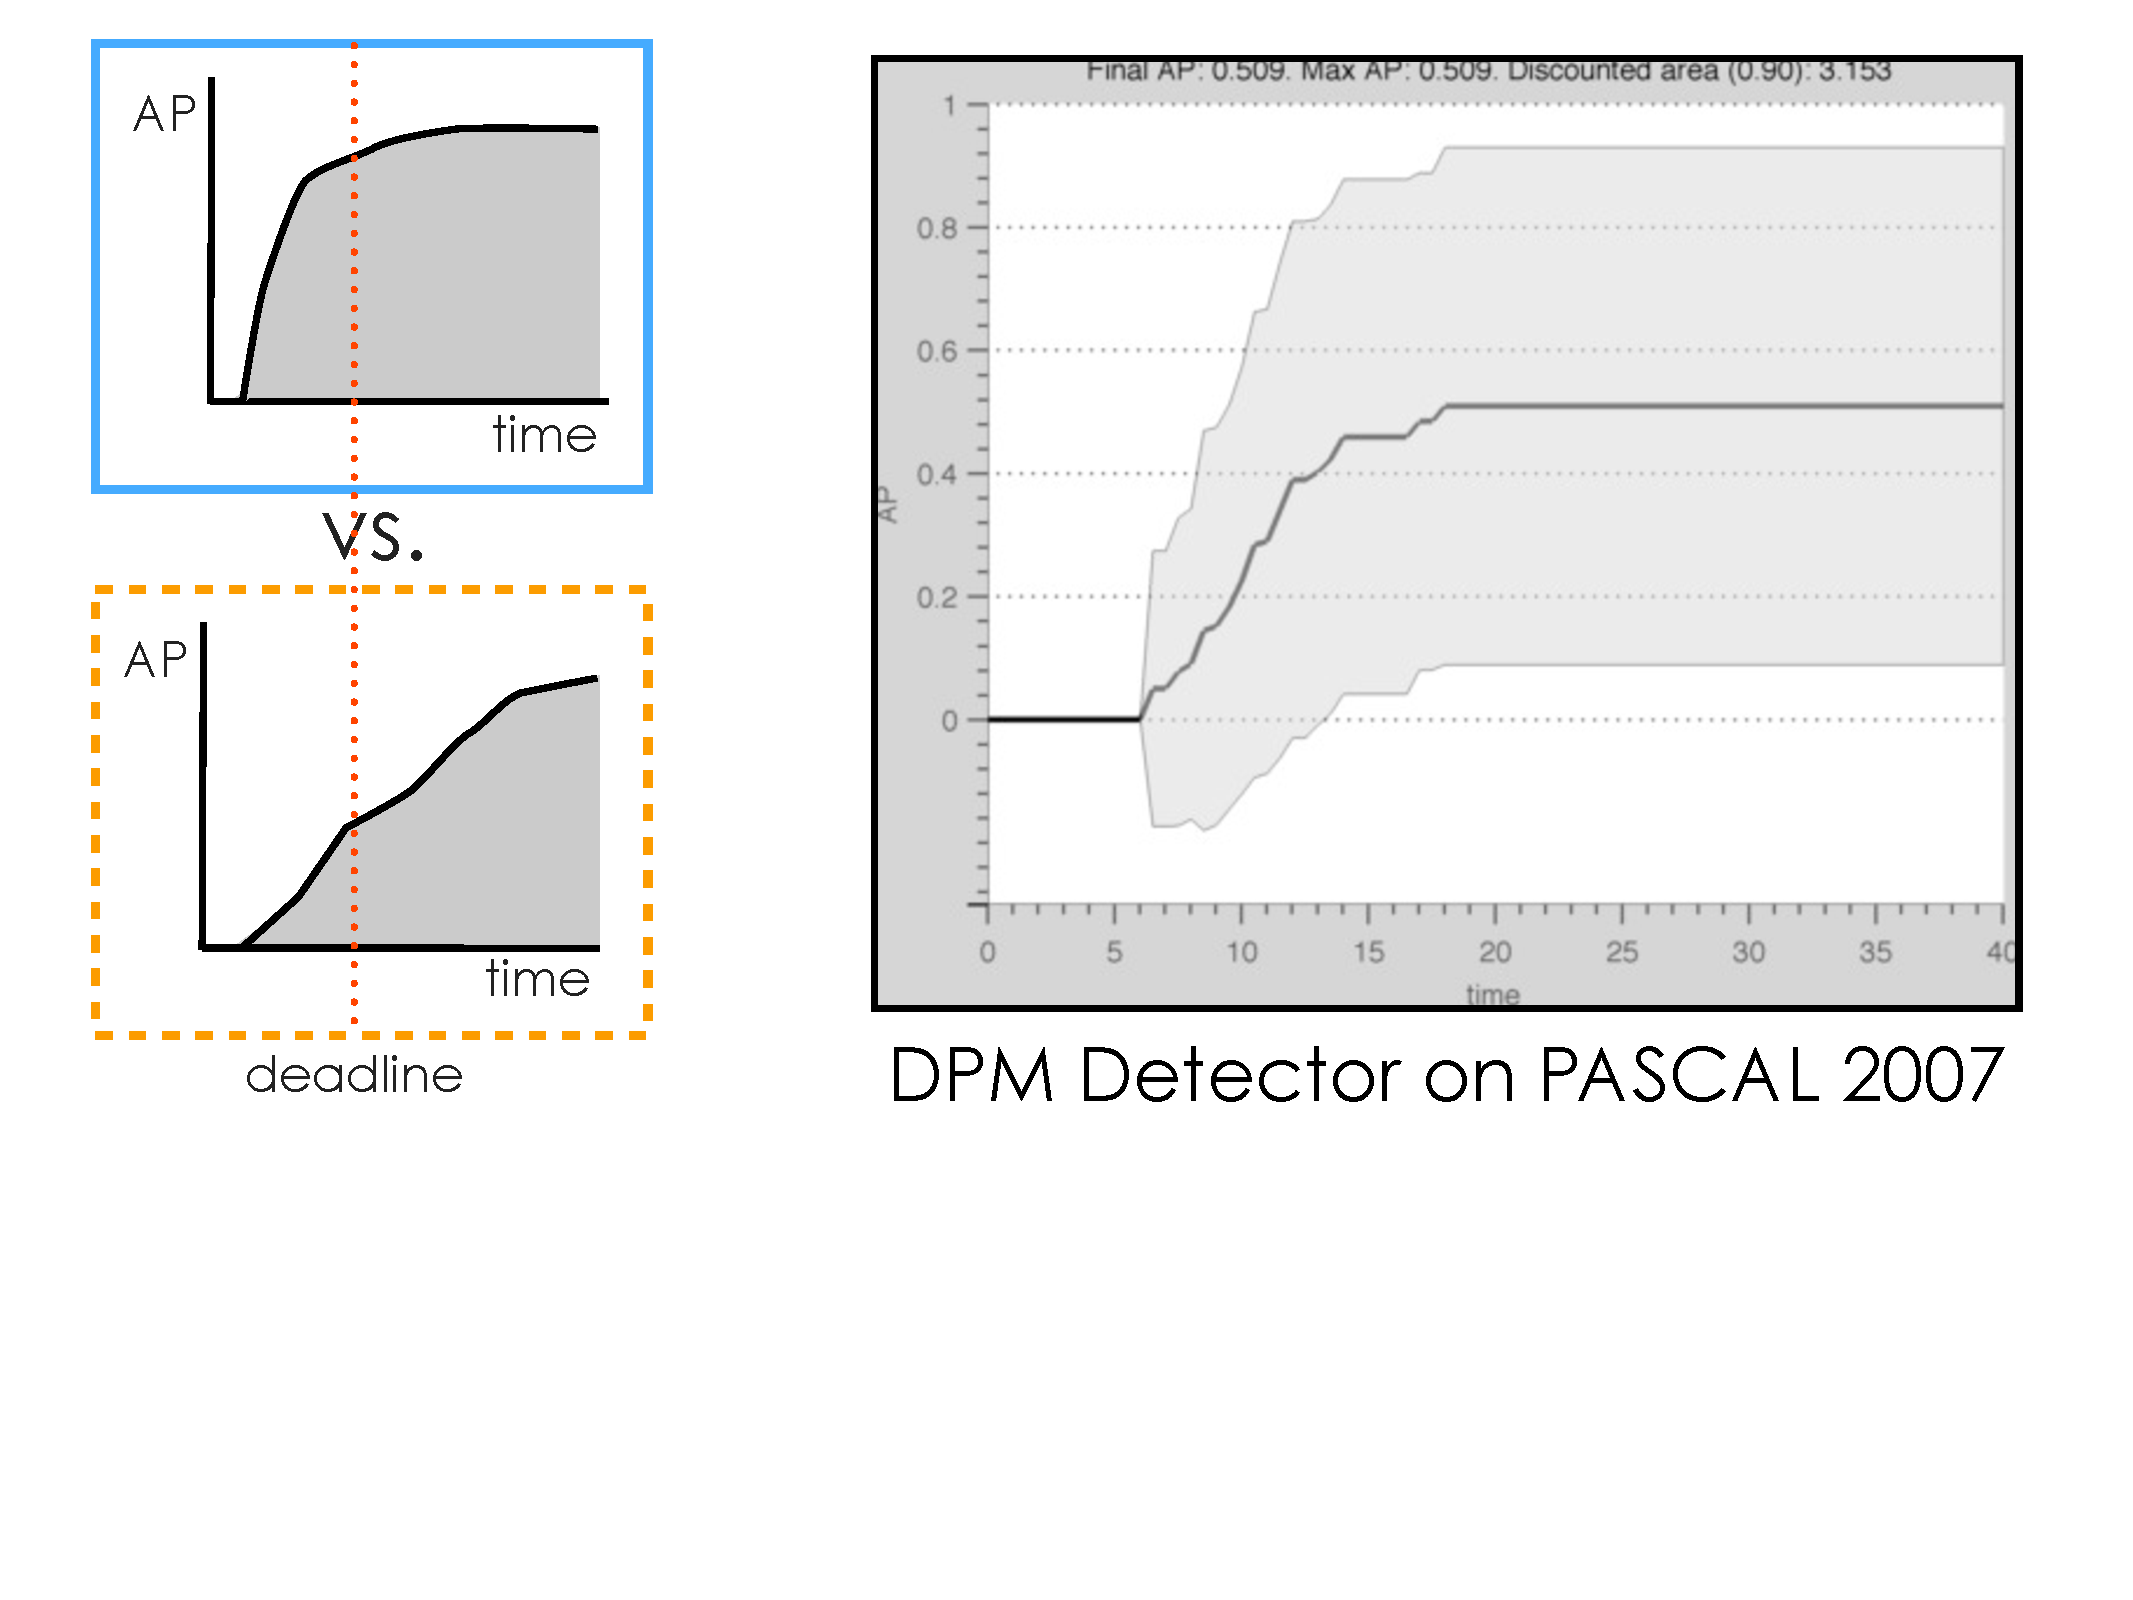
\includegraphics[width=22cm]{../../figures/budget.pdf}
      \end{center}
      
    \begin{itemize}
      \item Desired general behavior corresponds to maximizing the area under the Performance vs. Time curve: want the best performance as early as possible, after some setup time.
    \end{itemize}
    }; \addcenteredtitle{budget}{Budget: Performance vs. Time}

    % ==============================================================================
    \path (budget.south west) ++(0cm,-2cm) node(model) [style=tbox,text width=26cm] {
    \begin{itemize}
      \item We choose the next detection action (location and classifier) based on hypothesized contents of the image, inferred from previous detection actions.
    
      \item Window proposals follow a closed-loop policy in a partially observable decision process.
    \end{itemize}

    \begin{center}
      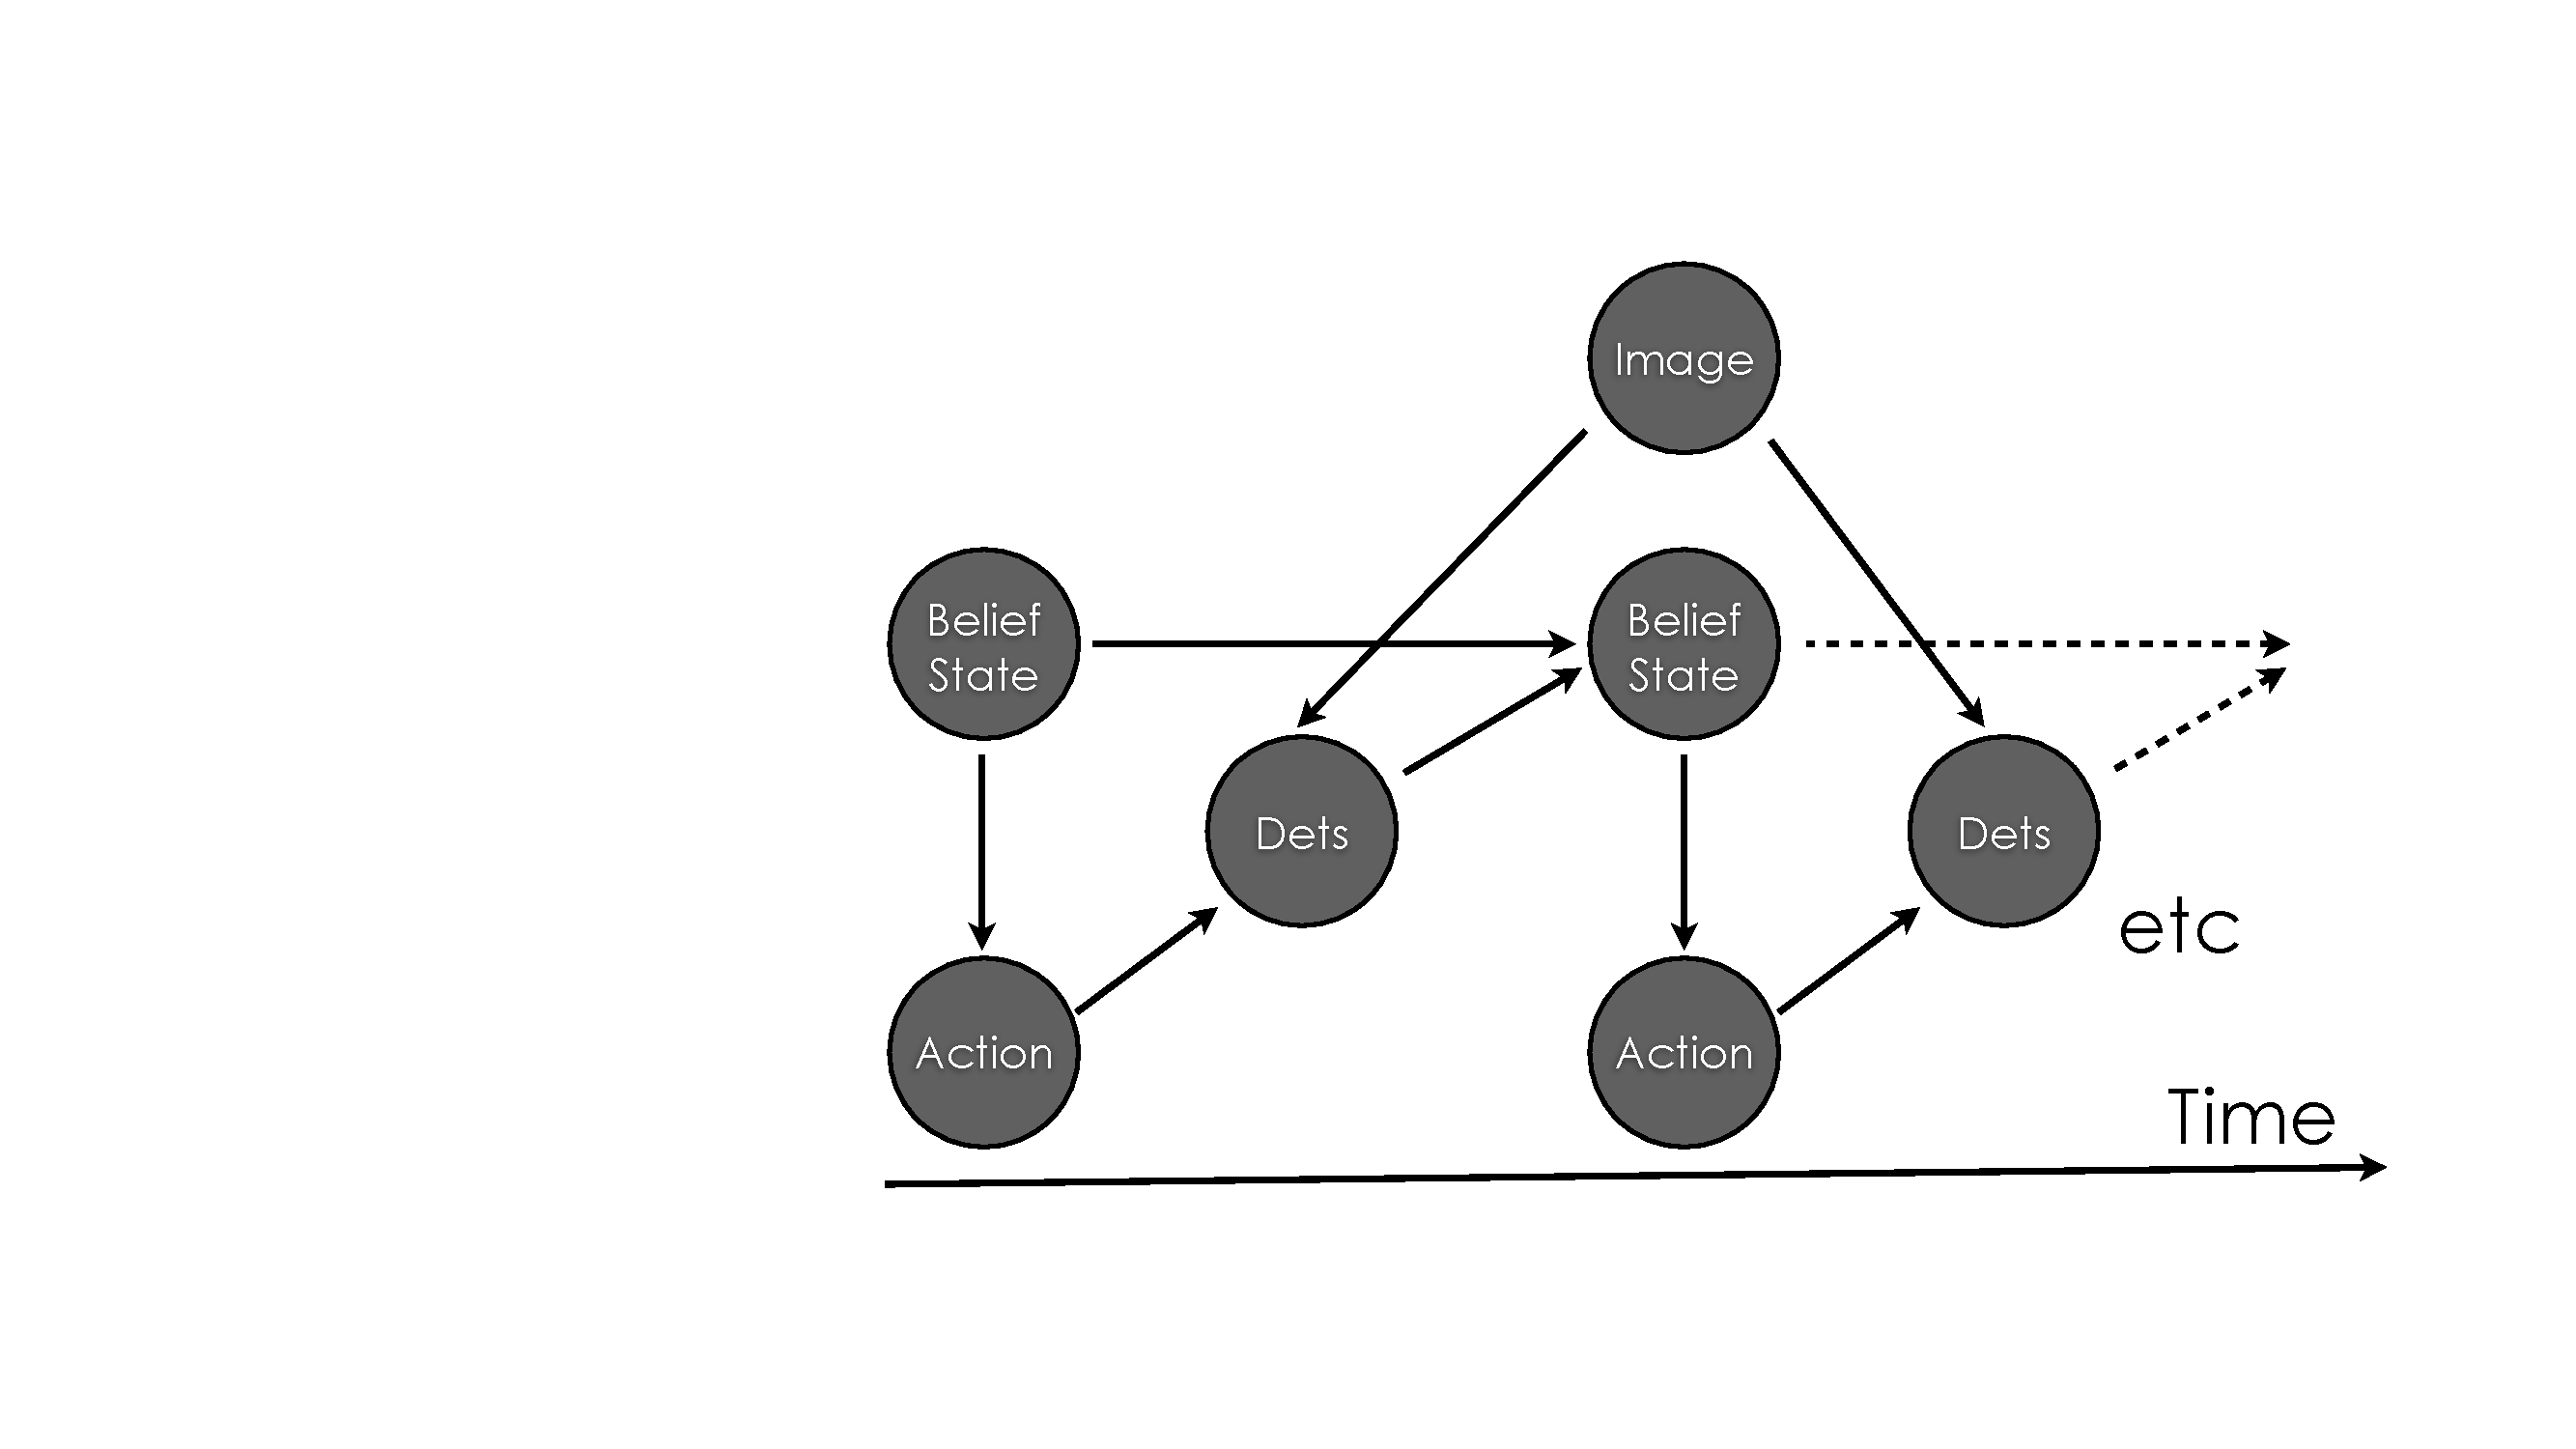
\includegraphics[width=16cm]{../../figures/pomdp.pdf}
    \end{center}

    {\bf Inferring state from detections}
    \begin{itemize}
      \item A detector is parametrized by two distributions $P(score|obj=true)$ and $P(score|obj=false)$.
      \item The likelihood of an object being in the window is inferred from these and the prior $P(obj=true)$.
    \end{itemize}
    }; \addcenteredtitle{model}{Our Approach}

    % ==============================================================================
    % RIGHT COLUMN
    \path (budget.north east) ++(2cm,0cm) node(cont) [style=tbox,text width=25cm] {
    {\bf Selecting action}
    \begin{itemize}
      \item The belief state consists of object posteriors for each class. These are treated as priors to the detection likelihoods.
      \item The AP can be predicted from these values, and forms our value function.
    \end{itemize}
    }; \addcenteredtitle{cont}{Our Approach, Continued}

    \path (cont.south west) ++(0cm,-2cm) node(results) [style=tbox,text width=25cm] {
    % ==============================================================================
    \begin{itemize}
      \item Currently evaluating state-of-the-art detectors in the AP-vs.-Time regime by modifying parameters such as stride or level of recall per cascade stage. 
    \item Initial experiments use a simple regression from set of detections so far to the value of running a given detector.
    \item ``Greedy'' oracle deemed a good enough target, so full reinforcement learning machinery is not used.
    \item Although it offers clear improvement, this scheme is not able to fully derive the signal in the data.
    \end{itemize}

    \begin{center}
      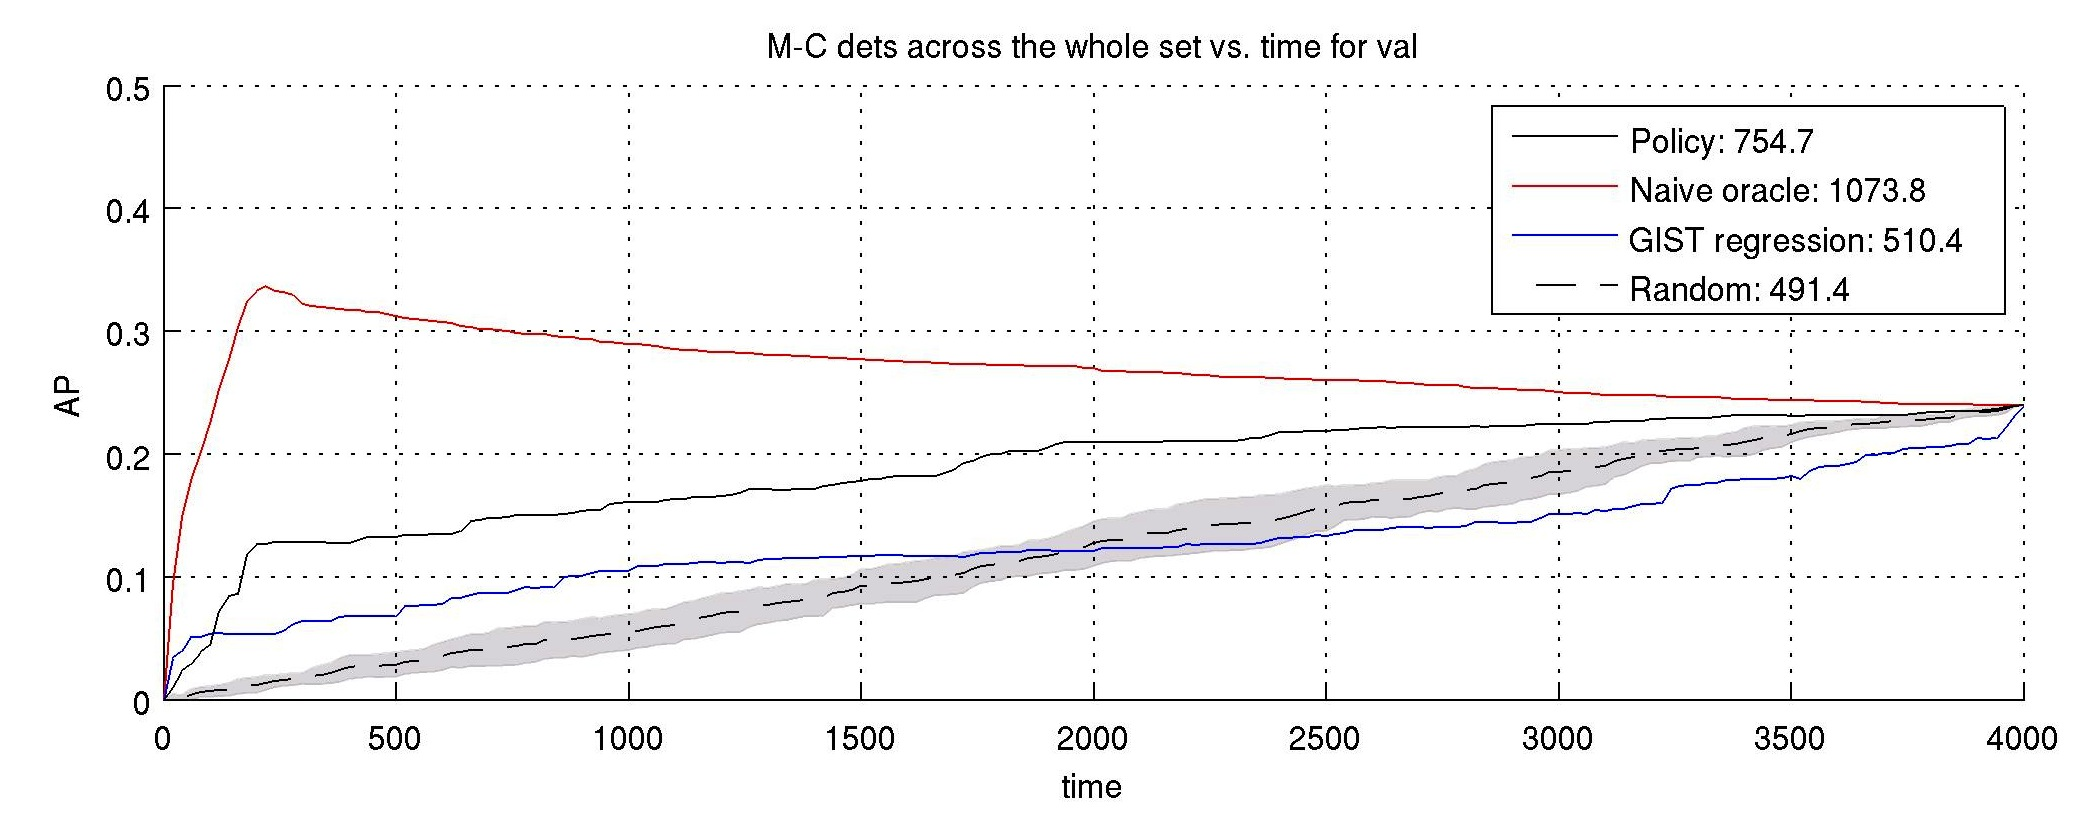
\includegraphics[width=23cm]{../../figures/result1.png}
    \end{center}

    }; \addcenteredtitle{results}{Results}

    % ==============================================================================
    \path (results.south west) ++(0cm,-2cm) node(opensource) [style=tbox,text width=25cm] {
      \begin{itemize}
      \item Research detection systems tend to be coded from scratch, wasting efforts---state-of-the-art systems are largely alike. Additionally, research detection systems commonly rely on MATLAB, which is prohibitively expensive for individuals and small companies.
      \item In the course of developing this project, we aim to make our Python implementation of a modularized detection system available open-source.
      \item We are working with OpenCV and PCL developers to provide a unified feature computation back-end to our system.
      \item Please visit http://object-detection.com for more info.
      \end{itemize}
    }; \addcenteredtitle{opensource}{Open Source Detection System}
\end{tikzpicture}

\end{center}
\end{document}

